\documentclass[a4paper]{article}
\setlength{\parindent}{0pt}

%%%%%%%% CREATE DOCUMENT STRUCTURE %%%%%%%%
%% Language and font encodings
\usepackage[english]{babel}
\usepackage[utf8x]{inputenc}
\usepackage[T1]{fontenc}
%\usepackage{subfig}

%% Sets page size and margins
\usepackage[a4paper,top=3cm,bottom=2cm,left=2cm,right=2cm,marginparwidth=1.75cm]{geometry}

%% Useful packages
\usepackage{framed}
\usepackage{amsmath}
\usepackage{graphicx}
%\usepackage[colorinlistoftodos]{todonotes}
\usepackage[colorlinks=true, allcolors=blue]{hyperref}
\usepackage{caption}
\usepackage{subcaption}
\usepackage{listings}
\usepackage{lstautogobble}
\usepackage{sectsty}
\usepackage{apacite}
\usepackage{float}
\usepackage{titling} 
\usepackage{blindtext}
\usepackage[square,sort,comma,numbers]{natbib}
\usepackage{xcolor}
\usepackage{algorithm}
\usepackage{forest}
\usepackage[noend]{algpseudocode}
\definecolor{darkgreen}{rgb}{0.0, 0.4, 0.0}

\definecolor{pblue}{rgb}{0.13,0.13,1}
\definecolor{pgreen}{rgb}{0,0.5,0}
\definecolor{pred}{rgb}{0.9,0,0}
\definecolor{pgrey}{rgb}{0.46,0.45,0.48}

\usepackage{listings}
\lstset{language=Java,
    showspaces=false,
    showtabs=false,
    breaklines=true,
    showstringspaces=false,
    breakatwhitespace=true,
    commentstyle=\color{pgreen},
    keywordstyle=\color{pblue},
    stringstyle=\color{pred},
    basicstyle=\ttfamily,
    colframe=white!75!black,
    moredelim=[is][\textcolor{pgrey}]{\%\%}{\%\%}
}

\usepackage[most]{tcolorbox}

\newtcblisting{shell}{colback=black,colupper=white,colframe=white!75!black,
	listing only,listing options={language=sh}}

% ToDo: List
\usepackage{enumitem,amssymb}
\newlist{todolist}{itemize}{2}
\setlist[todolist]{label=$\square$}


%%%%%%%% DOCUMENT %%%%%%%%
\begin{document}

%%%% Title Page
\begin{titlepage}

\newcommand{\HRule}{\rule{\linewidth}{0.5mm}} 							% horizontal line and its thickness
\center 
 
% University
\textsc{\LARGE University of Illinois @ Urbana-Champaign}\\[1cm]

% Document info
\textsc{\Large CI 487: Data Structures for CS Teachers}\\[0.2cm]
\textsc{\large }\\[1cm] 										% Course Code
\HRule \\[0.8cm]
{ \huge \bfseries Implementation \#5:\\\vspace{0.1cm}Generic AVL Tree}\\[0.7cm]								% Assignment
\HRule \\[0.8cm]
%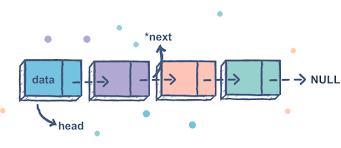
\includegraphics[width=0.6\textwidth]{images/singly-linked-list.png}\\[1cm] 	% University logo
\vfill 
\end{titlepage}

%%\begin{abstract}
%%Your abstract.
%%\end{abstract}

%%%% SECTIONS
%% Section 1
\section{Objectives }

The objectives of this assignment are as follows:
\begin{enumerate}
	\item Understand how to transform a BST into an AVL tree and the utility of doing so.
	\item Learn how to construct test cases and use the debugger in order to verify the AVL tree is being implemented correctly.
	\item Implement a novel recursive search algorithm that will report the number of steps to find a node in the tree.
\end{enumerate}

\section{Structures and Specifications}

\subsection{Step 0: Understanding the Code You're Given} 

The code you are given is quite similar to the BST starter code you were given last week with a few notable exceptions:
\begin{enumerate}
	\item \lstinline|TreeNode<E>|: The tree node class now contains a height attribute which you will use later in the assignment to keep track of that nodes height within the tree.
	\item \lstinline|inorderTraversal|: You are given a method that prints an in order traversal of the tree. This can be used to display the output of the tree in addition to verifying that your rotations aren't reordering the nodes in such a way that the BST rule is being broken.
	\item \lstinline|remove/findMinNode|: You are provided the BST remove method ad the findMinNode method. You will be modifying the former in step 1 in order to transform it into an AVL removal method.
	\item \lstinline|insert|: Your are also provided a working BST insertion method and, as was the case with remove, you will be transforming it into an AVL insert.
\end{enumerate}

As with all past assignments, it his recommended that you spend some time
reading the existing code in order to orient yourself before moving on to
the next step(s).

\subsection{Step 1: Modifying the BST Remove and Balance Methods}

The first step of our process of transforming a traditional BST into an AVL
tree is modifying the Insert and remove methods to include two things: 1) the
ability to update the heights of nodes as we recursively unwrap and 2) perform
rebalancing as the recursion unwraps. Below is the annotated psudeo code which
identifies the original portions from the BST class as well as the lines you
will add in order to accomplish the two tasks just described.

\begin{minipage}{0.49\textwidth}
    \begin{figure}[H]
        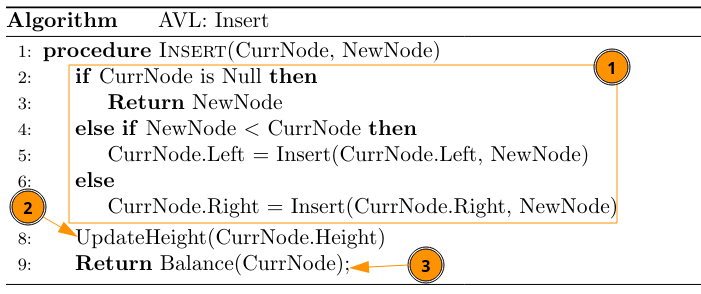
\includegraphics[width=\textwidth]{./images/avl-insert-annotate-algo.png}
    \end{figure}
\end{minipage}
\begin{minipage}{0.49\textwidth}
    \small
    \begin{enumerate}[1)]
        \item The first block is our usual insertion step. 
        \item If we have reached this line, we are performing the recursive unwrapping after inserting the node. Given we just inserted a node it is possible that the heights of the intermediary nodes we traversed over may need to have their height updated.
        \item Inserting a node may have caused the subtrees under the node we're on to come unbalanced so we should use the Balance method to rebalance if needed.
    \end{enumerate}
\end{minipage}

\begin{minipage}{0.49\textwidth}
    \begin{figure}[H]
        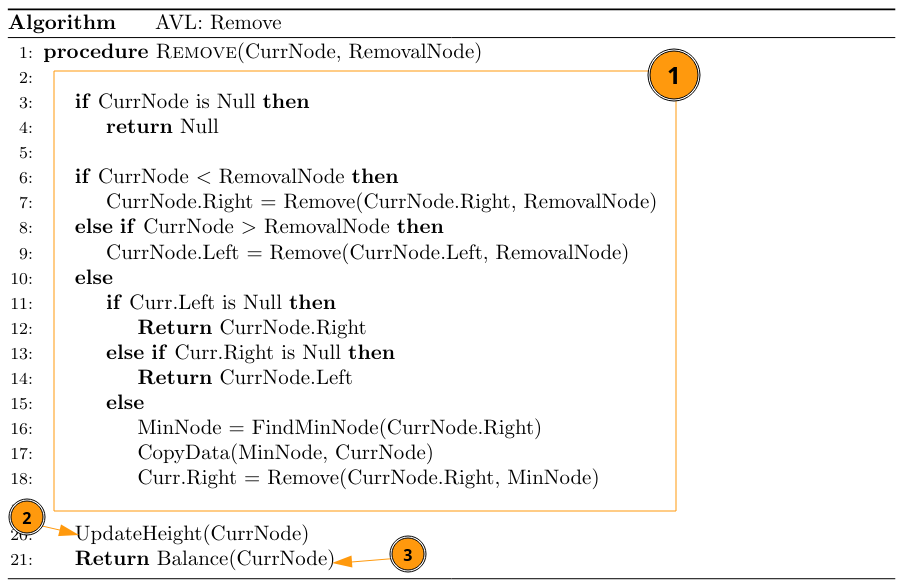
\includegraphics[width=\textwidth]{./images/avl-remove-algo-annotated.png}
    \end{figure}
\end{minipage}
\begin{minipage}{0.49\textwidth}
    \small
    \begin{enumerate}[1)]
        \item The first block is our usual insertion step. 
        \item After removing a node, the actual height of the node might have changed so we should update the current node's height.
        \item We should also call the balance method as removing a node might have caused a portion of the tree that was previously balanced to become unbalanced.
    \end{enumerate}
\end{minipage}
\vspace{0.2cm}\\
\textbf{Your Task:} Modify the existing recursive \lstinline|insert| and \lstinline|remove| methods to preform the height update and rebalancing steps detailed above. The equation for calculating the height of a node is as follows:
\[\text{Node.Height} = \text{Max(Node.Left.Height, Node.Right.Height)} + 1\]
Recall that, if a node isn't to the left or the right of a node, then we treat
it's height as $-1$.  Additionally, procedure for implementing the balance
method is detailed in the next section.\\

\textit{Hint:} At this point, it may be useful to create a method that takes a
reference to a node and returns -1 if it's null and it's height attribute if
its not.

\subsection{Step 2: The Balance Method}

\begin{minipage}{0.48\textwidth}
	\begin{algorithm}[H]
		\caption{AVL: Balance}\label{}
		\begin{algorithmic}[1]
			\Procedure{Balance}{N}
			\If{BF(N) $>$ 1}
			\If{BF(N.left) $<$ 0}
			\State N = RotateLeftRight(N)
			\Else
			\State N = Right(N)
			\EndIf
			\ElsIf{BF(N) $<$ -1}
			\If{BF(N.right) $>$ 0}
			\State N = RotateRightLeft(N)
			\Else
			\State N = Left(N)
			\EndIf
			\EndIf
			\State \textbf{Return} N
			\EndProcedure
		\end{algorithmic}
	\end{algorithm}
\end{minipage}
\hfill
\begin{minipage}{0.48\textwidth}
\textbf{Your Task:} Implement the balance method shown to the left. This method
will be the control center which will determine: 1) if the tree is unbalanced
with respect to $N$ and 2) select the correct rotation if rebalancing is
needed. It will do this using the balance factor which in turn uses height. The
equation for calculating balance factor is as follows:
\[BF(N) = N.Left.Height - N.Right.Height\]
Recall that, if a node isn't to the left or the right of a node then we treat it's height as $-1$.\\

\textit{Hint:} At this point, it may be useful to create a method that  can be
used to calculate the balance factor of a node.
\end{minipage}



\subsection{Step 3: Rotations}

\begin{minipage}{0.48\textwidth}
	\begin{algorithm}[H]
		\caption{AVL: Right Rotation}\label{}
		\begin{algorithmic}[1]
			\Procedure{Right}{N}
			\State Tmp = N.Left
			\State N.Left = Tmp.Right;
			\State Tmp.Right = N
			\State 
			\State UpdateHeight(N)
			\State UpdateHeight(Tmp)
			\State
			\State \textbf{Return} Tmp
			\EndProcedure
		\end{algorithmic}
	\end{algorithm}
\end{minipage}
\hfill
\begin{minipage}{0.48\textwidth}
	\begin{algorithm}[H]
		\caption{AVL: Left Rotation}\label{}
		\begin{algorithmic}[1]
			\Procedure{Left}{N}
			\State Tmp = N.Right
			\State N.Right = Tmp.Left;
			\State Tmp.Left = N
			\State 
			\State UpdateHeight(N)
			\State UpdateHeight(Tmp)
			\State
			\State \textbf{Return} Tmp
			\EndProcedure
		\end{algorithmic}
	\end{algorithm}
\end{minipage}
\\
\begin{minipage}{0.48\textwidth}
	\begin{algorithm}[H]
		\caption{AVL: LeftRightRotate}\label{}
		\begin{algorithmic}[1]
			\Procedure{LeftRightRotate}{N}
			\State N.Left = Left(N.Left)
			\State \textbf{Return} Right(N)
			\EndProcedure
		\end{algorithmic}
	\end{algorithm}
\end{minipage}
\hfill
\begin{minipage}{0.48\textwidth}
	\begin{algorithm}[H]
		\caption{AVL: RightLeftRotate}\label{}
		\begin{algorithmic}[1]
			\Procedure{RightLeftRotate}{N}
			\State N.Right = Right(N.Right)
			\State \textbf{Return} Left(N)
			\EndProcedure
		\end{algorithmic}
	\end{algorithm}
\end{minipage}
\\


\textbf{Your Task:} Implement each of the rotations using their respective psudeocode presented above.

\begin{enumerate}
    \item \lstinline|private TreeNode<E> leftRotate(TreeNode<E> node)|
    \item \lstinline|private TreeNode<E> rightRotate(TreeNode<E> node)|
    \item \lstinline|private TreeNode<E> leftRightRotate(TreeNode<E> node)|
    \item \lstinline|private TreeNode<E> rightLeftRotate(TreeNode<E> node)|
\end{enumerate}

It is recommended that you develop insertion test cases that you know will
trigger certain rotations and then investigate each method in the debugger in
order to: 1) verify that method is being called and 2) that the tree is being
properly updated.



\subsection{Step 4: Modified Search}

It can be tricky to verify whether or not an AVL tree is working correctly. One
way is to implement a method that calculates the number of steps it takes to
find a node in the tree. If you try to find one of the extreme values (i.e., leftmost/rightmost nodes)
and that operation takes around $log_2(N)$ steps to complete.\\

\textbf{Your Task:} You will be modifying your BST search method from last week. Rather than returning the node
that we found you will be returning the number of steps it took to find that node. For this exercise I \textbf{highly}
recommend Googling around to find similar problems and other solutions. The ability to break a problem down to several
keywords that yield existing answers that can be either directly used or modified is a highly useful skill and developing
that skill is a portion of the goal of this exercise.\\

For the provided test cases the numbers 1-10000 are inserted into an AVL tree. As such, your search operation should take 14
steps for both 1 and 10000 since they should be at the bottom of the tree and to the far right and far left, respectively..


\section{Checklist}
\begin{todolist}
    \item Read through all existing code in the files.
    \item Modify the following methods to update height and call balance:
    \begin{todolist}
        \item Insert
        \item Remove
    \end{todolist}
    \item Implement the Balance Method
    \item Implement the four rotations
    \begin{todolist}
        \item Left
        \item Right
        \item Left-Right
        \item Right-Left
    \end{todolist}
    \item Implement the modified search method.
	\item Construct test cases for each rotation (doesn't need to be turned in)
\end{todolist}
%%\newpage
%%\bibliographystyle{apacite}
%%\bibliography{sample}

\end{document}
